\documentclass[12pt,twoside]{article}

\usepackage[T1]{fontenc}
\usepackage[utf8]{inputenc}
\usepackage[spanish]{babel}

\let\layoutspanish\relax
\addto\captionsspanish{\def\tablename{Tabla}}
\unaccentedoperators

\usepackage[a4paper]{geometry}
  \geometry{hmargin={2.5cm,2.5cm},height=22cm}
  
\renewcommand{\baselinestretch}{1.2}  
\setlength{\partopsep}{0pt}
\setlength{\itemsep}{0pt}
\setlength{\topsep}{0pt}
\setlength{\parsep}{0pt}
\setlength{\parskip}{0.25\baselineskip}

\renewcommand{\textfraction}{0.1}
\renewcommand{\topfraction}{1}
\renewcommand{\bottomfraction}{1}
\renewcommand{\floatpagefraction}{1}

\setcounter{totalnumber}{5}
\setcounter{topnumber}{3}
\setcounter{bottomnumber}{2}

\usepackage{caption}
\setcaptionwidth{\textwidth}
\addtolength{\captionwidth}{-2\parindent}
\captionsetup{margin=\leftmargini,%
  width=\captionwidth,%
  labelfont={up,bf},%
  font={small,sl},%
  %indention={\captionindent
}

\usepackage{indentfirst}

\usepackage[pdftex]{color}

\usepackage[pdftex]{graphicx}

\usepackage{amsmath}
\allowdisplaybreaks 
\usepackage{amssymb}
\usepackage{amsfonts} 
\usepackage{enumerate}

\usepackage{fancyhdr}

\newcommand{\RunningAuthor}{Ginés Meca Carbonell}
\newcommand{\Author}[1]{\renewcommand{\RunningAuthor}{#1}}
\renewcommand{\leftmark}{\RunningAuthor}

\newcommand{\RunningTitle}{Métodos de Machine Learning basados en Árboles de Decisión.}
\newcommand{\Title}[1]{\renewcommand{\RunningTitle}{#1}}
\renewcommand{\rightmark}{\RunningTitle}

\pagestyle{fancy}
\fancyhf{}
\fancyhead[LO]{\small \slshape \leftmark}    
\fancyhead[RE]{\small \slshape \rightmark}   
\fancyhead[RO,LE]{\small \slshape \thepage}  

\renewcommand{\headrulewidth}{0.6pt}         
\renewcommand{\footrulewidth}{0pt}           
                                             
\setlength{\headheight}{1.5\headheight}      

\fancypagestyle{plain}{%                     
  \fancyhf{}                                 
  \setlength{\headwidth}{\textwidth}
  \fancyfoot[C]{\small \slshape \thepage}    
  \renewcommand{\headrulewidth}{0pt}
  \renewcommand{\footrulewidth}{0pt}
  }
  
\newcommand{\abs}[1]{\ensuremath{|#1|}}

\usepackage{hyperref}

\title{Métodos de Machine Learning basados en Árboles de Decisión}
\author{Ginés Meca Carbonell\\*[1em]
\begin{minipage}{0.75\textwidth}
\footnotesize \itshape
\begin{center}
Universidad de Alicante \\
4º de Grado en Matemáticas
\end{center}
\end{minipage}
}
\date{Junio 2022}

\usepackage{pdfpages}




\begin{document}


\includepdf[pages=1]{anexo-1-portada-memoria-tfg-matematicas.pdf}



\section*{Resumen}

\emph{En este trabajo, se ha estudiado el conjunto de algoritmos de Machine Learning derivados de los árboles de decisión.}

\newpage



\section*{Abstract}

\emph{}

\newpage



\tableofcontents



\newpage



\section{Introducción}

Vivimos en la era de la información. Cada segundo, millones de datos viajan entre diferentes lugares del planeta y se guardan formando enormes conjuntos de datos. Además, cada vez hay más instrumentos capaces de recoger información. Donde antes se necesitaba hacer uso de encuestas, ahora nos encontramos con dispositivos, como los teléfonos móviles, capaces de escribir texto, recoger audio y realizar fotografías y vídeos. Así, la información a nuestra alcance es infinita. Podemos conocer cuáles son los conceptos que son tendencia en los buscadores de internet, o cuáles son aquellos audiovisuales que más éxito están teniendo en las redes sociales. Del mismo modo, podemos acceder al historial de imágenes de la cámara de seguridad de nuestra vivienda o a la tabla que recoge las últimas operaciones de nuestra empresa. Es fácil obtener grandes cantidades de datos de aquello que nos interesa.

Dado que el número de datos que manipulamos cada vez es mayor,las técnicas utilizadas para analizarlos van evolucionando constantemente. Muchas de las técnicas clásicas del análisis de datos han quedado obsoletas, otras se utilizan para crear algoritmos más complejos. Uno de los algoritmos más conocidos es el de los árboles de decisión. Fueron introducidos por primera vez en 1963 por James N. Morgan y John A. Sonquist, quienes obtuvieron un método muy eficaz a través de un algoritmo muy básico. Actualmente, existen diferentes algoritmos que se pueden emplear a la hora de generar un árbol de decisión: CHAID, C4.5, FACT, QUEST, CRUISE... No obstante, el más conocido, y el que estudiaremos en este trabajo, es el algoritmo CART (Classification And Regression Trees), creado por Breiman, Friedman, Olshen y Stone en 1984. De hecho, fue el propio Leo Breiman quien, basándose en CART, desarrolló años más tarde el algoritmo Random Forest. Paralelamente, la publicación de Freund y Schapire en 1997 de un nuevo método basado en boosting daría lugar a otra serie de algoritmos; es aquí donde nos encontramos algoritmos más complejos, como el xgboost, que ocuparán gran parte del trabajo.

Dado que en los últimos años varios alumnos han realizado su TFG sobre árboles de decisión explicando su estructura más básica, resumiré las secciones dedicadas a ello con el fin de centrarme en analizar a fondo los algoritmos más complejos y novedosos que no se han tratado en estos trabajos y, así, elaborar un mapa conceptual de modelos lo más completo posible.



\subsection{Datos: Llueve en Australia} \label{sec: subsec11}

Para hacernos una idea de cómo funciona cada uno de los algoritmos detallados a lo largo del trabajo, haremos uso del conjunto de datos indicado. Se trata de un dataset en el que podemos encontrar mediciones de diferentes variables meteorológicas así como la fecha y localidad correspondientes y la información relativa a si llovió o no el día de la medición y el día siguiente.
\begin{figure}[h]
	\centering
	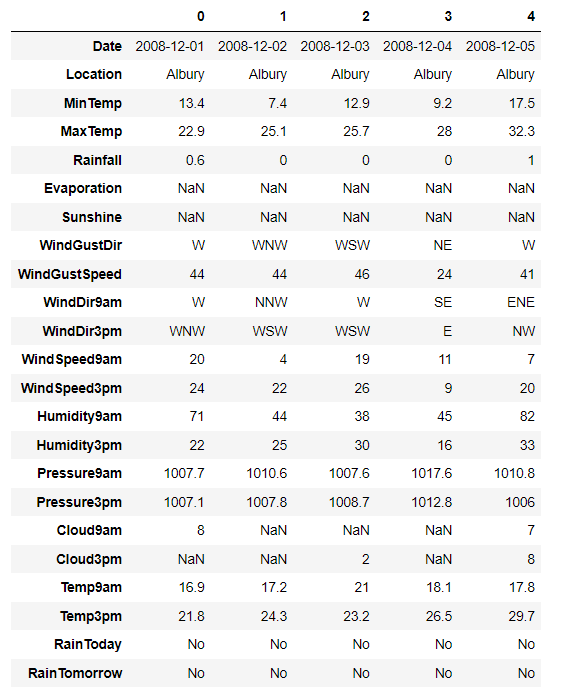
\includegraphics[width = 0.4\textwidth]{Intro_01}
	\caption{Encabezado del dataset}
\end{figure}

En total, se tiene 23 columnas que recogen información de 145460 días.


\subsection{Metodología}

A la hora de aplicar los diferentes métodos al conjunto de datos se procederá mediante validación cruzada. Es decir:

\begin{enumerate}
\item Se selecciona el modelo correspondiente.
\item Se separa, al azar, el conjunto de datos inicial en dos: datos de entrenamiento y datos de testeo.
\item Se entrena el modelo con los datos de entrenamiento.
\item Se aplica el modelo entrenado a los datos de testeo.
\item Se comprueba la veracidad de las predicciones realizadas.
\end{enumerate}

Habitualmente, la división del conjunto inicial que da lugar a los subconjuntos de entrenamiento y testeo se realiza de manera aleatoria. No obstante, dada la naturaleza de los datos, procederemos de otra manera.

Separando el conjunto de datos de manera aleatoria nos encontraremos con que los datos de testeo se encontrarán intercalados con los de entrenamiento. Esto puede ocasionar que la predicción de testeo a realizar se encuentre entre dos datos utilizados al entrenar el modelo. Este método no es erróneo, pero no nos da ninguna información acerca de cómo se desenvuelve el algoritmo a la hora de clasificar datos de fechas posteriores.

Entonces, el procedimiento será ligeramente distinto, emplearemos la validación 'Out Of Time'. Dado que nuestro dataset contiene fechas desde el 01/11/2007 hasta el 24/06/2017, nuestro conjunto de entrenamiento estará formado por todos aquellos datos con fecha anterior al 01/01/2015 y los datos de testeo serán los restantes. Así, entrenamos el modelo con datos anteriores a los de testeo para saber cómo van a ser las predicciones futuras y asemejarnos más a lo que nos interesaría en un caso real: entrenar el modelo de manera que al introducir las fechas actuales, no registradas, y de las cuales no sabemos que ocurrirá unos días o semanas más tarde en función de los datos que poseemos sobre fechas posteriores.

Además, los cálculos se realizarán en el lenguaje de programación Python. Todo el código se encuentra disponible en el Anexo (\ref{sec:Anexo}).



\newpage



\section{Árboles de decisión CART}
\subsection{Preliminares}

Los árboles de decisión son muy utilizados como método predictor (tanto de regresión como de clasificación) dada su simpleza, su efectividad y lo visual que resulta su funcionamiento a través de un gráfico, lo cual facilita su comprensión. Se trata de un algoritmo que divide sucesivamente el conjunto inicial de datos en diferentes subconjuntos a través de diversas condiciones relacionadas con sus variables explicativas. Por ejemplo:

\textbf{Ejemplo 2.1: } \textit{Se pretende estudiar la variable 'RainTomorrow' del conjunto de datos dado en función de las variables explicativas 'Cloud3pm' y 'Humidity3pm'(nivel de nubosidad y de humedad a las 15.00, respectivamente) para predecir si lloverá o no al día siguiente. Así, escogiendo únicamente las variables explicativas indicadas, el esquema que seguirá nuestro árbol de clasificación será el siguiente: }
\begin{figure}[h]
	\centering
	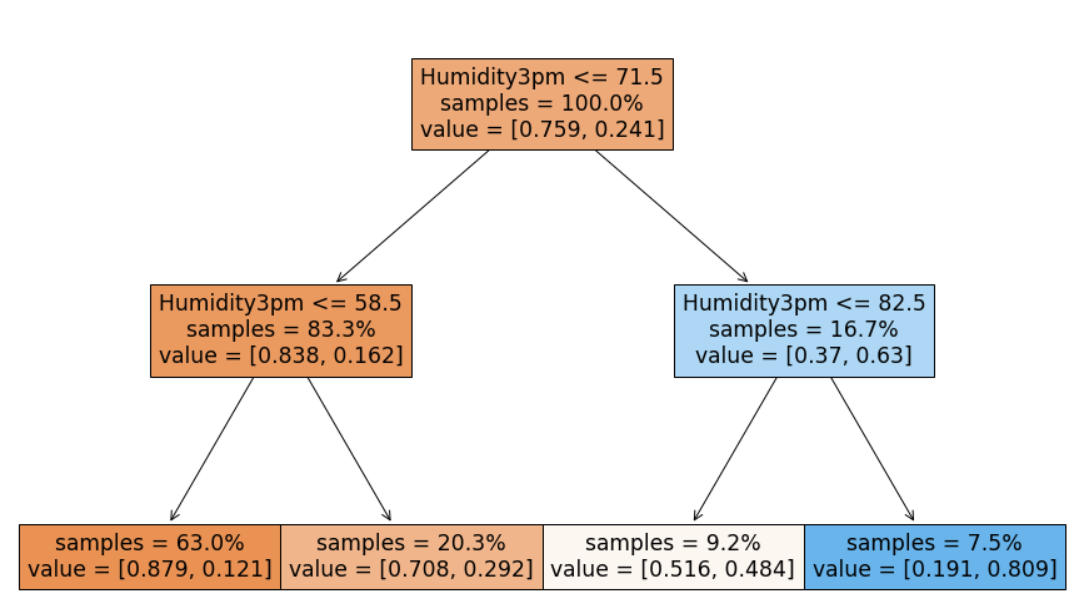
\includegraphics[width = 0.7\textwidth]{ex2_1_01}
	\caption{Ejemplo 2.1. Árbol de decisión}
	\label{fig:Ejemplo 2.1}
\end{figure}

Como se puede observar, el algoritmo es muy intuitivo: se introduce un individuo y se le aplica la primera condición; si la respuesta es afirmativa se sigue el camino de la izquierda y si es negativa el de la derecha. Mediante este proceso, se va comprobando si sus variables explicativas cumplen las diferentes condiciones que se plantean hasta llegar a un grupo que deja de dividirse, que será su predicción.

Por otro lado, es fácil ver que las condiciones del algoritmo se corresponden con particiones del espacio. Como en el ejemplo anterior se han elegido únicamente dos variables explicativas, se puede hacer una representación de los individuos sobre $\mathbb{R}^{2}$ y determinar sobre él las diferentes regiones de predicción.
\begin{figure}[h]
	\centering
	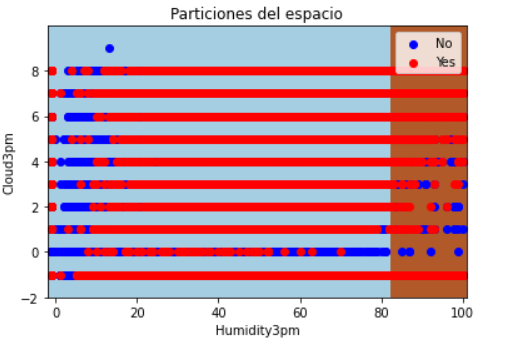
\includegraphics[width = 0.5\textwidth]{ex2_1_02}
	\caption{Partición del espacio del Ejemplo 2.1}
	\label{fig:Ejemplo 2.1.2}
\end{figure}


\subsubsection{Notación y conceptos básicos}

A continuación, se introducirán una serie de términos básicos para poder hacer referencias correctas a los conceptos presentados. Por un lado, nos encontramos con las siguientes definiciones:
\begin{description}
\item[Nodo raíz: ]Primer nodo, que contiene a todos los individuos, a partir del cual comienzan a realizarse las divisiones.
\item[Nodo interno: ]Nodos intermedios que provienen de una división y desencadenan otra. Dentro de ellos, se pueden definir:
	\begin{description}
	\item[Nodo padre: ]Nodo anterior a un nodo interno fijado.
	\item[Nodos hijos: ]Nodos resultantes de la división del nodo interno fijado.
	\end{description}
\item[Nodo hoja: ]Nodos finales que dan lugar a la predicción.
\end{description}

Se pueden identificar todos estos nodos en la figura del ejemplo 2.1 (\ref{fig:Ejemplo 2.1}). Se tienen un nodo raíz, seis nodos internos y 8 nodos hoja.

Por otro lado, conviene hablar del concepto de sobreajuste (en inglés: overfitting). Se dice que un modelo se encuentra sobreajustado si el algoritmo se ha adaptado en exceso a los individuos del conjunto de entrenamiento. Este hecho provoca que la predicción de los individuos de este conjunto sea muy buena, mientras que al introducir nuevos individuos estas predicciones presentan grandes errores.

Para lidiar con el sobreajuste, interesa manejar también otras dos nociones: el sesgo y la varianza. El sesgo (en inglés: bias) hace referencia a los errores cometidos en las predicciones de los individuos de nuestro conjunto de entrenamiento. Por contra, la varianza es la medida del error cometido en los individuos que no pertenecen a este conjunto; en nuestro caso, lo mediremos en los individuos del conjunto de testeo. No obstante, estos conceptos generan un problema: interesa tener valores bajos de ambos indicadores, pero disminuir el sesgo conlleva un aumento de la varianza. Así, a la hora de construir un modelo de Machine Learning, interesa estudiar que el sesgo no sea excesivamente bajo, para evitar el sobreajuste, pero también que no sea excesivamente alto para que las predicciones sean fiables.


\subsubsection{Objetos de estudio de un CART}

Una vez visto cómo se realizan las predicciones al trabajar con árboles de decisión, corresponde explicar el funcionamiento del mismo. Para ello, habrá que tratar los siguientes aspectos:
\begin{enumerate}
\item Elección de variables y valores asociados a cada nodo interno.
\item Criterio de parada de división de los nodos
\item Valor o clase asignada a cada nodo
\end{enumerate}


\subsection{Elección de variables y valores asociados a cada nodo interno} \label{sec: subsec22}
Sea un conjunto de datos de n individuos y p+1 variables ($n,p \in \mathbb{N}$). De este modo, sean $X_1, X_2, ... , X_p$ las variables explicativas e $y$ la variable dependiente. En el caso de nuestro conjunto de datos de ejemplo:
\begin{table}[h]
\centering
\begin{tabular}{rcccc|c}
 & \multicolumn{1}{l}{$X_1$}         & $X_2$                        & ...                      & $X_{22}$ & $y$ \\ \hline
\multicolumn{1}{l|}{$x_1$} & \multicolumn{1}{r|}{2008-12-01} & \multicolumn{1}{l|}{Albury} & \multicolumn{1}{l|}{...} & No        & \multicolumn{1}{l|}{No} \\ \hline
\multicolumn{1}{l|}{$x_2$} & \multicolumn{1}{r|}{2008-12-02} & \multicolumn{1}{l|}{Albury} & \multicolumn{1}{l|}{...} & No        & \multicolumn{1}{l|}{No} \\ \hline
\multicolumn{1}{l|}{$x_3$} & \multicolumn{1}{r|}{2008-12-03} & \multicolumn{1}{l|}{Albury} & \multicolumn{1}{l|}{...} & No        & \multicolumn{1}{l|}{No} \\ \hline
\end{tabular}
\end{table}

Pese a las similitudes existentes entre los árboles de regresión y los de clasificación, conviene dividir este apartado en dos con tal de mostrar el funcionamiento exacto de cada uno de ellos.


\subsubsection{Árboles de regresión}
Se busca conocer cómo realizar las divisiones. En particular, nos centraremos en la primera división y el proceso será similar para las siguientes. Al situarnos en el nodo raíz, nos encontramos con el conjunto de datos al completo y pretendemos dividirlo en dos regiones, que denotaremos $R_1$ y $R_2$, en función de una de las variables explicativas, $X_j$, y de un valor respecto de esta, s, de manera que:
\begin{equation*}
R_1 (j,s) = \{ X | X_j \leq s \} \, \, \, \wedge \, \, \,  R_2 (j,s) = \{ X | X_j > s\}
\end{equation*}

Sabemos que $Y_1$ se mantendrá constante sobre $R_1$ y que $Y_2$ también será constante sobre $R_2$. De esta manera, buscamos j y s tales que:
\begin{equation*}
\min_{j,s}(\min_{c_1, c_2}(\sum_{x_i \in R_1}(y_i - c_1)^2 + \sum_{x_i \in R_2}(y_i - c_2)^2))
\end{equation*}
o lo que es lo mismo, buscamos j y s que minimicen el error cometido en la predicción de los individuos del conjunto de entrenamiento. Esta tarea se puede llevar a cabo probando todos los casos posibles y escogiendo el que minimice la expresión.


\subsubsection{Árboles de clasificación}
En el caso de los árboles de clasificación, la variable dependiente es una clase; es decir, como en la tabla dada al comienzo de la subsección (\ref{sec: subsec22}). Ahora, en lugar del error mínimo cuadrático, introduciremos una función de impureza que nos permita evaluar la homogeneidad de los nodos; es decir, que nos permita estudiar qué acciones separan mejor el espacio en función de las diferentes clases. El criterio más empleado es el índice Gini, que se define como:
\begin{equation*}
G_{region} = \sum_{k=1}^K p_{mk}(1 - p_{mk})
\end{equation*}
donde $p_{mk}$ es la proporción de individuos del conjunto de entrenamiento de clase k que se encuentran en la región m y K es el número total de clases. Así, fijado un m, se puede calcular el índice Gini de una determinada región. Además, se puede observar que valores de $p_{mk}$ cercanos a 0 o 1 implican que el producto $p_{mk}(1- p_{mk})$ sea muy pequeño. Por tanto, el índice Gini actúa como medidor de la pureza de una región: un índice Gini bajo significa que los diferentes $p_{mk}$ están cercanos a 0 o 1 y la región es "pura".

Sabiendo esto, solo queda evaluar el índice Gini de un nodo. Esto se hace mediante una media ponderada, es decir:
\begin{equation*}
G_{nodo} = \frac{n_1}{n_1 + n_2}G_1 + \frac{n_2}{n_1 + n_2}G_2
\end{equation*}
donde  $n_1$ y $n_2$ son la cantidad de individuos de las regiones $R_1$ y $R_2$, respectivamente, y $G_1$ y $G_2$ son los índices Gini de las mismas. Así, la tarea se resume en obtener, mediante comprobación de todas las opciones posibles, la variable y el valor que minimizan el índice Gini del nodo.




\subsection{Criterio de parada de escisión de nodos}
Se podría pensar que la precisión de un CART aumenta conforme aumenta en profundidad, es decir, conforme aumenta en número de particiones. No obstante, como ya se ha introducido, cuantas más particiones del espacio realice el algoritmo, más se estará ajustando a los datos del conjunto de entrenamiento, lo que puede llevar a sobreajuste. Con tal de evitar este hecho, se han implementado algunos métodos de "poda" del árbol. Es evidente que podando el árbol se introduce sesgo, pues no dejamos que se adecue totalmente a los datos de entrenamiento; sin embargo, haciendo esto de manera controlada se consigue disminuir la varianza y mejorar las predicciones.

Por un lado, la técnica más simple consiste en establecer una profundidad máxima. Con esta condición, se puede asegurar que los nodos dejarán de dividirse una vez alcanzado el nivel indicado. Por ejemplo, en el Ejemplo 2.1 (Figura \ref{fig:Ejemplo 2.1}) se ha establecido una profundidad máxima igual a 3.

Por otro lado, el árbol determinará un nodo como nodo hoja cuando la separación del mismo no sea conveniente en términos de pureza. El procedimiento es el siguiente: en primer lugar, se calcula el índice Gini de la región asociada a ese nodo y, después, se realiza la división del nodo y se calcula el índice Gini del mismo(proveniente de la media ponderada de índices de sus regiones). Si el índice de la región sin dividir es inferior al índice del nodo, se deshará la división y se determinará el nodo como nodo hoja, pues de esta manera se mantiene una mayor pureza.


\subsection{Valor o clase asignada a cada nodo hoja}
Como se comentaba anteriormente, el resultado de un árbol de decisión es una partición del espacio. Supongamos que se obtienen M regiones diferentes denotadas por $R_{m}$ con $m = 1, ..., M$. Por tanto, definamos como Y al árbol de decisión y como $c_m$, con $m = 1,...,M$, a las predicciones (imágenes de Y) asociadas a cada región $R_m$. De este modo:
\begin{equation*}
Y(x) = \sum^M_{m = 1} c_{m}I(x \in R_m) \, \, \, \forall x \in D
\end{equation*}
donde D es el dominio de la función (espacio de las variables explicativas) e I es la función indicadora:
\begin{equation*}
I(x) = 
\left.
\begin{array}{ccc}
1 & si & x \in R_m \\
0 & si & x \not\in R_m 
\end{array}
\right\}
\end{equation*}


Así, a la hora de entrenar un modelo, se busca minimizar los errores entre y e Y. Por ejemplo, si tomamos el error mínimo cuadrático, llegamos al problema:
\begin{equation*}
\min_{Y_i} \sum_{i=1}^n (y_i - Y_i)^2 \Rightarrow \min_{c_m} \sum_{m = 1}^M \sum_{x_i \in R_m} (y_i - c_m)^2
\end{equation*}
donde $Y_i = Y(x_i) \, \, \forall i=1,...n$. Si denotamos $f(c_m) = \sum_{x_i \in R_m} (y_i - c_m)^2$, observamos que alcanzar la solución óptima del problema planteado es equivalente a minimizar la función f:
\begin{equation*}
f'(c_m) = -2 \sum_{x_i \in R_m} (y_i - c_m) = -2 \sum_{x_i \in R_m}y_i + 2n_mc_m = 0 \Leftrightarrow c_m = \frac{1}{n_m} \sum_{x_i \in R_m}y_i
\end{equation*}
y
\begin{equation*}
f''(c_m) = -2 \sum_{x_i \in R_m} (-1) = 2n_m > 0
\end{equation*}
donde $n_m$ es el conjunto de datos pertenecientes a la región $R_m$, $\forall m = 1,...M$.

En conclusión, el valor asignado a cada nodo hoja será la media de las observaciones de los individuos del conjunto de entrenamiento que pertenecen a dicho nodo.

En el caso de árboles de clasificación, la tarea se simplifica: basta con calcular la proporción de individuos de cada clase en cada región y, así, el valor asignado a cada subconjunto del espacio será la clase a la que le corresponde la mayor proporción en el mismo.


\subsection{Ejemplo}
\textit{Se desea obtener una predicción fiable acerca de las precipitaciones del día siguiente en una ciudad de Australia. Para ello, haciendo uso del dataset anteriormente introducido, se dividirá el conjunto de datos en dos subconjuntos: uno de entrenamiento y otro de testeo. Además, probaremos con diferentes profundidades máximas permitidas para así construir el árbol más fiable.}

\textit{Además, con tal de analizar los resultados, utilizaremos el AUC; es decir, el área bajo la curva ROC('Area Under the Curve'), creada en base a la sensibilidad(tasa de  verdaderos positivos) y especifidad(tasa de verdaderos negativos) de las predicciones. Así, operando el AUC de la forma $2 \times AUC - 1$ obtenemos el coeficiente Gini(no confundir con el índice Gini de escisión de nodos). Cuanto más alto sea el valor de este coeficiente, mejor será nuestro clasificador.}

\textit{Con esto, aplicando los diferentes árboles de clasificación, llegamos al siguiente resultado:}

\begin{figure}[h]
\centering
\includegraphics[width = 0.3\textwidth]{ex2_2_01}
\caption{Resultados árboles de clasificación para RainTomorrow}
\end{figure}

\textit{En la tabla se ven reflejados los coeficientes de Gini para los conjuntos de entrenamiento y testeo y el porcentaje de información que se pierde en el conjunto de testeo respecto del de entrenamiento.}

\textit{Como podemos observar, cuando la profundidad máxima permitida es superior o igual a 10, el modelo empieza a sobreajustarse a los datos de entrenamiento aumentando, conforme aumenta la profundidad, la desviación entre los conjuntos. Es decir, el bias se reduce pero la varianza se dispara. Así, los modelos más fiables son el $DT\_3$ y el $DT\_5$ (profundidades 3 y 5) pues en ambos la variación se encuentra por debajo del $5\%$.}

\textit{El valor $delta\%$ se puede entender como desviación que sufre el conjunto de testeo con el paso de 2 años (recordemos que los datos de testeo van de 2015 a 2017). Por tanto, si escogiésemos un modelo con un $delta\% = 20\%$, tendríamos que este $20\%$ se iría incrementando en nuestras predicciones cada dos años, algo que llevaría a un modelo totalmente impreciso. Por ello, escogemos aquellos con variaciones pequeñas.}



\subsection{Ventajas y desventajas}
Como ya avanzábamos, y como hemos podido observar a través del ejemplo, los árboles de decisión son una herramienta muy potente para el análisis de datos. No obstante, pese a presentar muchos puntos a favor, también hay una serie de inconvenientes a tener en cuenta. En esta subsección, nos encargaremos de analizarlos.

\textbf{\underline{Ventajas:}}
\begin{itemize}
\item Se pueden emplear en problemas de regresión y de clasificación.
\item Es un método muy intuitivo de fácil comprensión.
\item La manera de proceder del modelo se asemeja a cómo lo hace la mente humana: se van estableciendo condiciones que restringen, paso a paso, el conjunto total de datos hasta llegar a la solución.
\item Se puede obtener una representación gráfica de los diferentes modelos, lo cual facilita su comprensión a nivel visual.
\end{itemize}

\textbf{\underline{Desventajas:}}
\begin{itemize}
\item La capacidad predictora de los árboles de decisión es inferior a la que se puede obtener mediante otros métodos. De hecho, podemos observar que la fiabilidad del modelo del ejemplo anterior en el conjunto de testeo no alcanza el $65\%$.
\item Se trata de un algoritmo inestable. Es decir, un ligero cambio en los datos de entrenamiento puede conllevar a la creación de un modelo totalmente distinto. %¿Por qué?
\end{itemize}



\newpage
\section{Métodos derivados de los árboles de decisión}
Los árboles de decisión son una gran herramienta predictiva. Tanto los CART como muchos de los algoritmos utilizados para construir árboles de decisión se desarrollaron a lo largo de la década de los 80. No obstante, ya hemos visto que estos algoritmos no llegan a alcanzar grandes niveles de eficacia; por tanto, durante la década de los 90 se publicaron diferentes artículos con distintas técnicas que, utilizando árboles de decisión, consiguen aumentar con creces estos niveles de fiabilidad.

A la hora de combinar los árboles de decisión para construir modelos más complejos se pueden seguir dos caminos: bagging o boosting.


\subsection{Algoritmos de bagging}
Los algoritmos de bagging se caracterizan por tomar muestras aleatorias del conjunto de datos inicial y construir con ellas árboles de decisión. De esta manera, se generarán tantos árboles como muestras se hayan tomado. Así, la respuesta de un algoritmo de bagging en un problema de regresión será el promedio de las respuestas de cada uno de los árboles y en un problema de clasificación será la clase que más veces se ha repetido.

Analizaremos tres algoritmos de bagging distintos: Bagging, Random Forest y Extra-Trees.


\subsubsection{Bagging}
Tras participar en la creación del algoritmo CART, Leo Breiman publicó, en 1996, un artículo en el que introducía un nuevo método con el fin de disminuir la varianza de CART: Bagging. Bagging es un algoritmo que toma diferentes muestras aleatorias de individuos con repetición del conjunto de datos y con cada una de ellas construye un árbol de decisión haciendo uso de todas las variables explicativas disponibles.


\subsubsection{Random Forest}
El desarrollo de Bagging llevó a Breiman a definir un nuevo algoritmo 5 años más tarde. Con Random Forest, Breiman consiguió, además de disminuir la varianza, obtener información más completa de las variables explicativas. El procedimiento es muy parecido al de Bagging: nuevamente se toman diferentes muestras con repetición de los individuos y, para cada muestra, también se toma una muestra aleatoria de m variables (con $m \leq p$). Una buena elección de m podría ser: $ m = \lfloor \sqrt{p} \rfloor$.

De esta manera, cada árbol presentará diferentes variables explicativas; lo que se traduce en árboles con variables significativas totalmente distintas, pues aquellas que lo son para un árbol puede ser que no se encuentren en el siguiente.


\subsubsection{Extra-Trees}
El algoritmo Extra-Trees, o Extremely Randomized Trees, aporta aún más margen a la aleatoriedad dentro del modelo. Utiliza como base lo descrito en Random Forest y a la hora de realizar las escisiones de nodos en cada árbol, asigna un valor aleatorio a cada variable. Así, a la hora de realizar una partición del espacio no se debe probar con todos los valores posibles para cada una de las p variables, se probará con m valores generados aleatoriamente correspondientes a las m variables explicativas.


\subsubsection{Ejemplo}
\textit{Nuevamente, se desea predecir si lloverá o no el próximo día en una ciudad de Australia. Para ello, usaremos el conjunto de datos que ya hemos utilizado con anterioridad y aplicaremos los diferentes algoritmos de bagging vistos en la subsección con el fin de compararlos y comentar sus mejoras. Además, con tal de evitar sobreajustes, estableceremos el criterio de parada de los árboles generados en 5 (como se ve en el ejemplo de CART, es el más fiable junto a 3) y probaremos con diferentes números de árboles generados por cada algoritmo.}

\textit{Al igual que en el ejemplo de CART, calcularemos el índice Gini haciendo uso del AUC para elegir los modelos más precisos y realizar correctamente las comparaciones.}

\textit{Aplicando los diferentes algoritmos llegamos a: }

\begin{figure}[h]
\centering
\includegraphics[width = 0.9\textwidth]{ex3_1_01}
\caption{Resultados algoritmos de bagging para RainTomorrow}
\end{figure}

\noindent
\textit{donde 'Bag' se corresponde con Bagging, 'RT' con Random Forest y 'ET' con Extra-Trees. Como se puede apreciar, la mejora respecto a CART es evidente: en el ejemplo anterior llegamos a la conclusión de que una de las mejores opciones era elegir el árbol con profundidad máxima 5 que nos otorgaba un índice Gini de 0.655905 en el conjunto de entrenamiento y de 0.626416 en el de testeo. Ahora, escogiendo los modelos que generan 100 árboles ($Bag\_100$, $RF\_100$ y $ET\_100$), obtenemos índices de Gini que rozan, en ocasiones, el 0.7 en ambos conjuntos además de un significante descenso, de aproximadamente 1 punto, en delta$\%$, lo cual refleja un claro descenso de la varianza.}


\subsubsection{Ventajas y desventajas}
Al igual que se ha hecho con CART, a continuación se realizará un análisis de pros y contras de los algoritmos de bagging.

\textbf{\underline{Ventajas:}}
\begin{itemize}
\item Los algoritmos de bagging son capaces de disminuir la varianza; lo que implica que las predicciones realizadas serán (casi) igual de fiables que las del conjunto de entrenamiento.
\item Los algoritmos de bagging son más precisos que otros algoritmos más simples (como CART).
\end{itemize}

\textbf{\underline{Desventajas:}}
\begin{itemize}
\item Se pierde la fácil visualización y el entendimiento de CART.
\end{itemize}


\newpage
\subsection{Algoritmos de boosting}
Los algoritmos de boosting, al igual que los de bagging, generan diferentes árboles de decisión a través de los cuales se realiza la predicción final. No obstante, mientras los algoritmos de bagging generan árboles independientes y devuelven una respuesta promedio o la respuesta más votada, los algoritmos de boosting generan los árboles secuencialmente, teniendo en cuenta los resultados anteriores. De esta manera, esta clase de métodos consigue reducir el sesgo; es decir, el error cometido en los datos del conjunto de entrenamiento, ya que la forma en la que se construyen los diferentes CART permite otorgar pesos diferentes a los individuos, consiguiendo así que el nuevo árbol generado se focalice en predecir bien a aquellos individuos que presentan mayor error (o que se han clasificado erróneamente) en el árbol anterior.

A lo largo de esta subsección trataremos de abordar a fondo los principales algoritmos de boosting: AdaBoost, Gradient Boosting, XGBoost, LightGBM y CatBoost.


\subsubsection{AdaBoost}
Adaboost fue publicado en 1997 por Freund y Schapire. El algoritmo es el siguiente:
\begin{figure}[h]
\centering
\includegraphics[width = 0.8\textwidth]{AdaBoost_01}
\caption{The Elements of Statistical Learning}
\label{fig: AdaBoost_01}
\end{figure}

A continuación, procederemos a explicarlo con detalle.

Partimos de una matriz de datos X compuesta por n individuos a los que se les miden p variables. Además, disponemos de la variables dependiente, que denotaremos por y. Además, como ya avanzábamos, AdaBoost construye los árboles secuencialmente modificando los pesos de los individuos en cada iteración; por tanto, también habrá que tener en cuenta la matriz de pesos. Es decir:
\begin{equation*}
X =
\begin{pmatrix}
x_{11} & x_{12} & \dots & x_{1p} \\
x_{21} & x_{22} & \dots & x_{2p} \\
\vdots & \vdots & \ddots & \vdots \\
x_{n1} & x_{n2} & \dots & x_{np} 
\end{pmatrix}
\, \, \, 
\wedge
\, \, \,
y = 
\begin{pmatrix}
y_1 \\
y_2 \\
\vdots \\
y_n
\end{pmatrix}
\, \, \,
\wedge
\, \, \,
P =
\begin{pmatrix}
w_1 & 0 & \dots & 0 \\
0 & w_2 & \dots & 0 \\
\vdots & \vdots & \ddots & \vdots \\
0 & 0 & \dots & w_n
\end{pmatrix}
\end{equation*}

Como podemos ver en la figura \ref{fig: AdaBoost_01}, el primer paso consiste en asignar el mismo peso a todos los individuos; ya que no se ha realizado ningún árbol previo y, por tanto, nos interesa calcular buenas predicciones del máximo número de individuos posibles. Así, en primer lugar:
\begin{equation*}
w_i = \frac{1}{n} \, \, \, \forall i \in \{1, \dots, n \}
\end{equation*}

A continuación, siguiendo el esquema de la figura \ref{fig: AdaBoost_01}, se crea un árbol de decisión. Una particularidad de AdaBoost es que, en lugar de árboles al uso, construye tocones; es decir, algoritmos que solo contienen dos nodos hoja. De esta manera, cada tocón construido (denotados por $G_m$) realiza una única división del espacio, obteniendo dos subconjuntos. Además, es evidente que en cada tocón únicamente se verá involucrada una variable.

Una vez construido el tocón, siguiendo los métodos explicados en la subsección \ref{sec: subsec22}, definimos:

\begin{equation*}
err_m = \frac{\sum_{i=1}^{n} w_i I(y_i \neq G_m(x_i))}{\sum_{i=1}^{n} w_i} 
\end{equation*}

\noindent
es decir, la suma de los pesos de los individuos mal clasificados en el numerador y la suma de los pesos en el denominador. La expresión del denominador nos permite asegurar que $err_m \in [0, 1]$, ya que con las modificaciones que se aplicarán posteriormente, la suma $\sum_{i = 1}^n w_i$ puede ser distinta de 1 para alguna de las iteraciones posteriores. Notemos que, para $m = 1$:

\begin{equation*}
err_1 = \frac{\sum_{i=1}^{n} w_i I(y_i \neq G_1(x_i))}{\sum_{i=1}^{n} w_i} = \frac{\frac{1}{n} \sum_{i=1}^{n}I(y_i \neq G_1(x_i))}{1} = \frac{num.errores}{n}
\end{equation*}

A continuación, siguiendo el apartado 3b de la figura \ref{fig: AdaBoost_01}, definimos:

\begin{equation*}
\alpha _m = \log \left( \frac{1 - err_m}{err_m} \right)
\end{equation*}

Teniendo en cuenta que $err_m \in [0, 1]$, podemos dibujar la gráfica de la función $\alpha_m$:





\newpage
\section{Anexo} \label{sec:Anexo}
Todo el código empleado en la elaboración de los ejemplos se encuentra en la carpeta de GitHub creada para tal fin (\url{link})

En cuanto a los datos utilizados, como ya se comenta en la introducción (\ref{sec: subsec11}), han sido extraídos de Kaggle y se puede llegar a ellos a través del siguiente link: \url{https://www.kaggle.com/jsphyg/weather-dataset-rattle-package}.

Además, se ha realizado un procesamiento de los mismos para su correcta utilización. Para ello, se ha seguido la siguiente estructura, la cual se encuentra disponible en la web de Kedro (\url{https://kedro.readthedocs.io/en/stable/12_faq/01_faq.html}):
\begin{figure}[h]
\centering
\includegraphics[width = \textwidth]{Kedro}
\caption{Figuras disponibles en el link de Kedro.}
\end{figure}
\end{document}